Bursting dynamics has been extensively studied in a wide variety of neural systems, as it is instrumental for many brain functions, including motor coordination and cognitive performance, and can be related to both healthy and pathological states. Neuronal models in computational neuroscience often reproduce key functional features of their biological counterparts. However, they also present limitations such as their poor ability to mimic the observed intrinsic variability of living neurons, particularly in membrane potential waveforms and in collective adaptive dynamics. Biophysical models typically produce stereotyped fixed membrane potential depolarization and repolarization waveforms, and restricted dynamical flexibility as compared to those observed in experimental recordings. Variability in the activity of living neurons has been proven to play an important role in relevant information processing tasks. We have seen in this chapter, the importance of variability in the presence of sequential dynamical invariants in the bursting activity and the limitations of studying them in a model when the variability is induced by a current ramp stimulation. The variability in models has usually been induced by gaussian noise, but this ignores the importance of the functional variability in the neurons, the observed variability is not only a cause of stochastic alterations but a functional outcome. 

In this section, we will describe this variability characteristics in experimental recordings, not only regarding the sequence time-intervals but also their waveforms. We will compare this variability with that of classical models and models able to produce chaotic activity. 
Figure \ref{fig:lp-pd burst variability} shows examples of the bursting and waveform variability in the intracellular recordings of LP and PD neurons in the pyloric CPG of \textit{Carcinus maenas}. In both neurons, we can appreciate a wide variability in the burst shape and duration, including the variability in the hyperpolarization.

\begin{figure}[hbt]
	\centering
	\begin{minipage}{0.48\textwidth}
		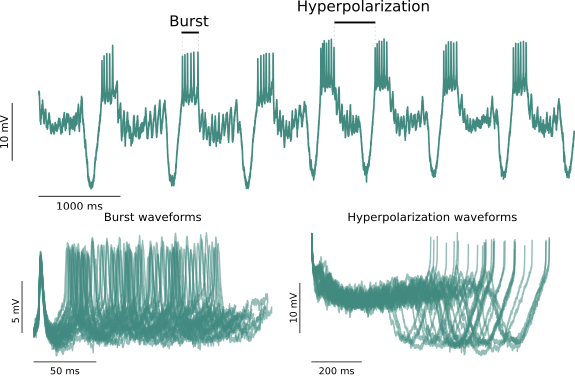
\includegraphics[width=\textwidth]{img/invariants/variability/lp_burst_variability.png}
	\end{minipage}
	\begin{minipage}{0.48\textwidth}
		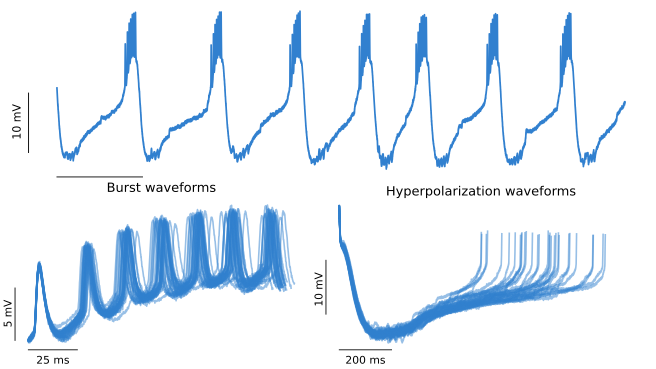
\includegraphics[width=\textwidth]{img/invariants/variability/pd_burst_variability.png}
	\end{minipage}
	\caption{Example of variability in waveforms from intracellular recordings of the LP and PD neurons in the pyloric CPG}
	\label{fig:lp-pd burst variability}
\end{figure}

Although models can faithfully reproduce the activity and shape of neural models, they usually fail on reproducing the intrinsic and collective variability that we observe in electrophysiological recordings, this is the case for example of \textcite{hodgkin_quantitative_1952} or \textcite{vavoulis_dynamic_2007}, represented in Fig. \ref{fig:model burst no variability}. In that reproduction, although the waveform shape is accurate, the functional variability is hindered, reproducing a tonic and steady bursting activity. 

\begin{figure}[hbt]
	\centering
	\begin{minipage}{0.48\textwidth}
		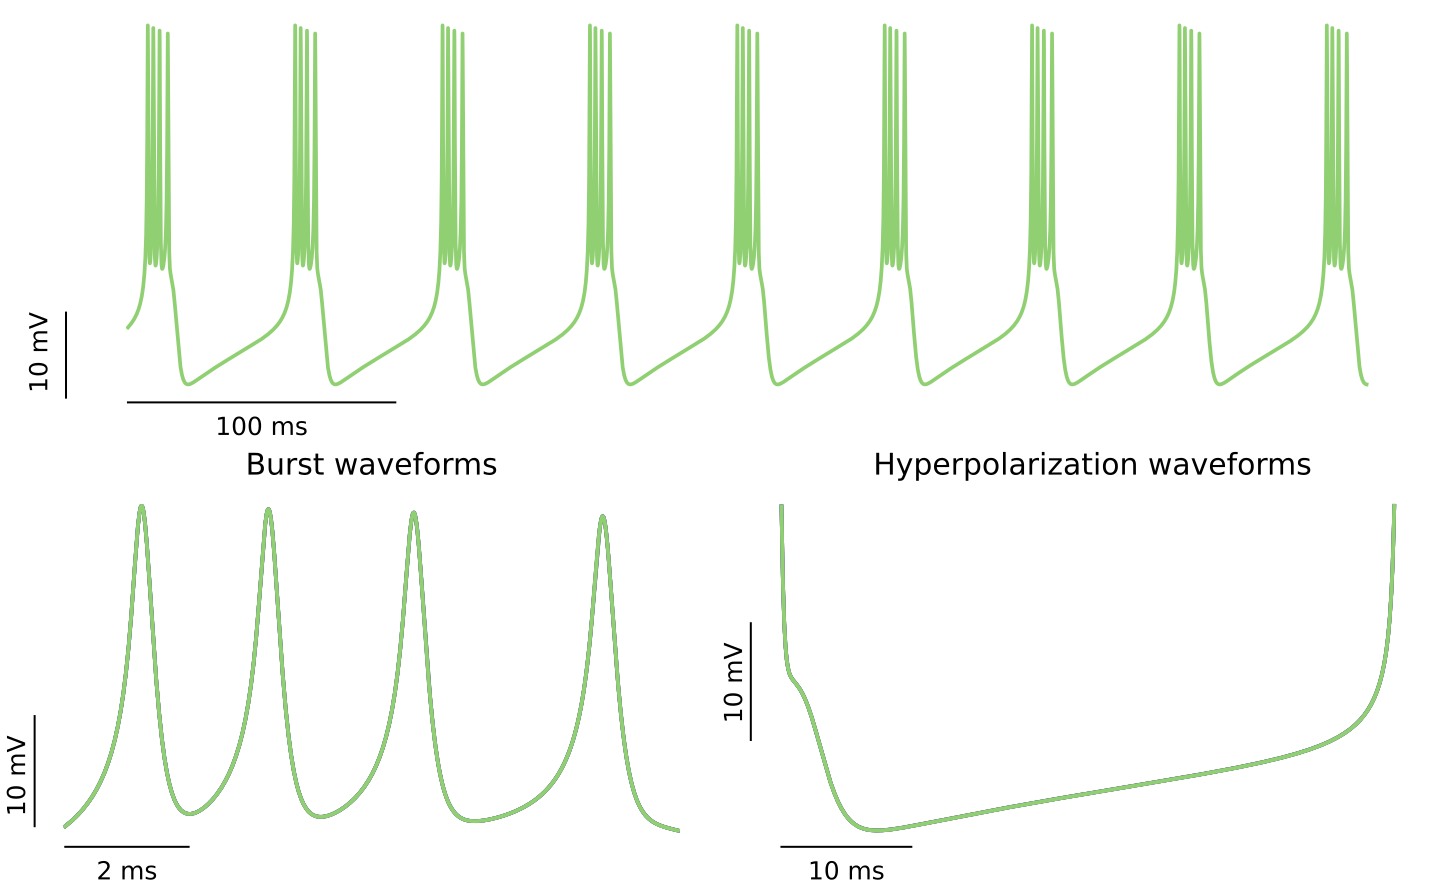
\includegraphics[width=\textwidth]{img/invariants/variability/GHmodel.png}
	\end{minipage}
	\begin{minipage}{0.48\textwidth}
		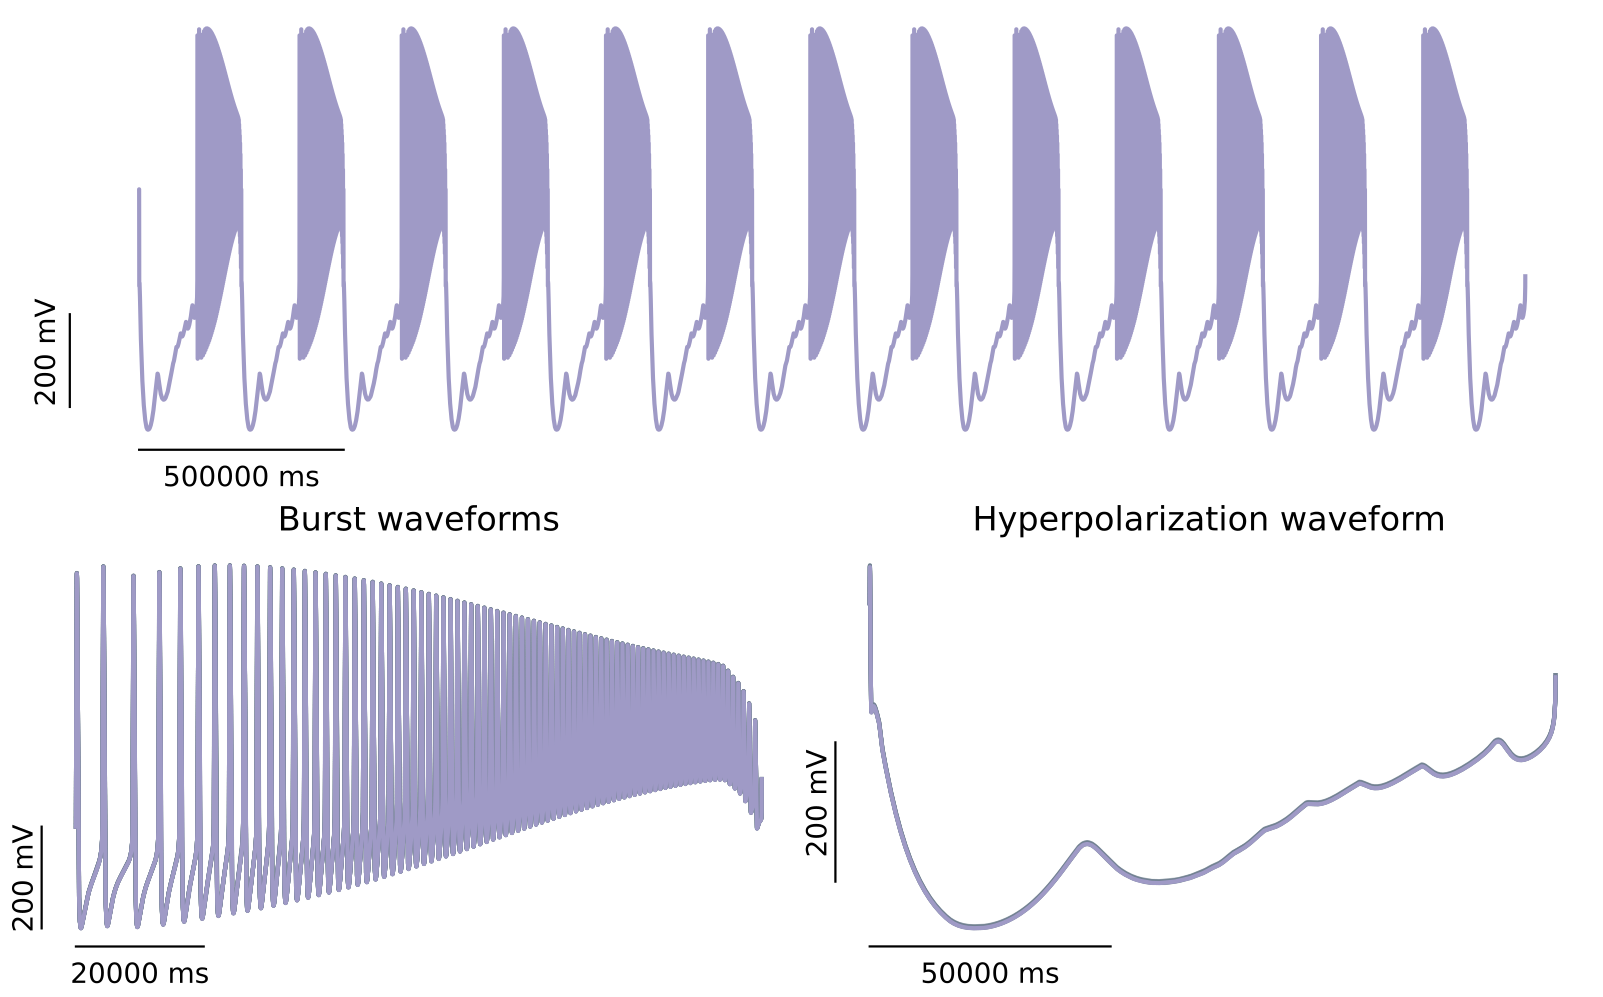
\includegraphics[width=\textwidth]{img/invariants/variability/N1Mnovar.png}
	\end{minipage}
	\caption{Example of bursts with no variability in waveforms from model simulation of neuron from \textcite{ghigliazza_minimal_2004b} model in chaotic mode and N1M neuron from \textcite{vavoulis_dynamic_2007} with no ramp stimulation in the CPG circuit. The equations for both models can be found in Secs. \ref{sec:model variability equations} and \ref{sec:CPG model equations}, respectively.}
	\label{fig:model burst no variability}
\end{figure}



In section \ref{sec:CPG model equations}, we saw that variability can be induced by including a current ramp, although it can reproduce the variability, when studying the activity cycle-by-cycle it hinders the functional variability of the spontaneous activity. 


\begin{figure}[hbt]
	\centering
	\begin{minipage}{0.48\textwidth}
		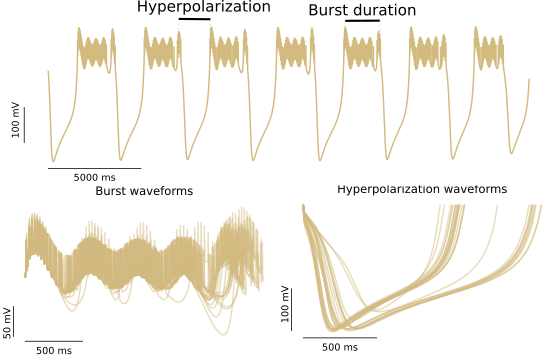
\includegraphics[width=\textwidth]{img/invariants/variability/TN-burst_variability.png}
	\end{minipage}
	\begin{minipage}{0.48\textwidth}
		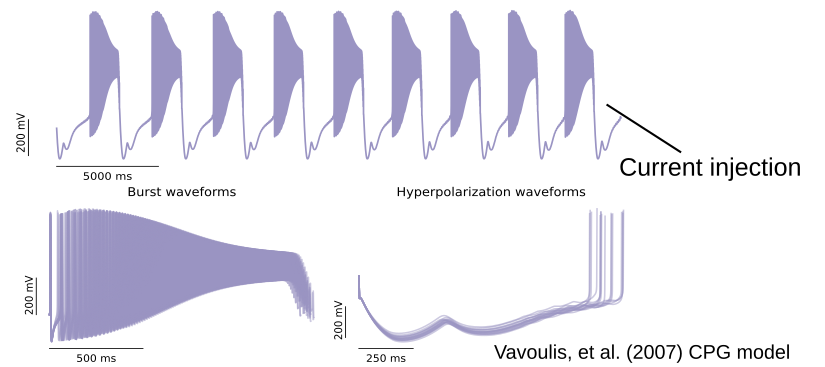
\includegraphics[width=\textwidth]{img/invariants/variability/n1m_vav_burst_variability.png}
	\end{minipage}
	\caption{Example of variability in waveforms from model simulation of neuron from \textcite{nowotny_probing_2008} model in chaotic mode and N1M neuron from \textcite{vavoulis_dynamic_2007} under current stimulation in the CPG circuit. The equations for both models can be found in Secs. \ref{sec:model variability equations} and \ref{sec:CPG model equations}, respectively.}
	\label{fig:model burst variability}
\end{figure}


Modern experimental techniques involving activity-dependent electrical, optical and chemical stimulation can further unveil and explain functional variability of bursting sequences in a wide variety of nervous systems, it is important to rely on models able to reproduce the intrinsic variability. It will also be relevant for designing associated applications in the context of neurotechnology, artificial intelligence and robotics \parencite{garrido-pena_exploring_2024}. 

%
%In this work, we illustrate that current biophysical neuron models fail to reproduce the intrinsic and collective variability observed in electrophysiological recordings in the nervous system of different animals, and how this hinders the theoretical study of the relevance of sequential neural dynamics. We also assess the solution to this problem in well-known bursting neuron models by identifying possible biophysical and synaptic candidates that can explain the observed variability while sustaining the robustness of the model oscillatory activity. Finally, we discuss the importance of model intrinsic variability in the context of biohybrid circuits built with interacting living and model neurons to evaluate the role of robust sequential neuronal and circuit dynamics in motor function coordination.

%Bursting dynamics has been extensively studied in a wide variety of neural systems, as it is instrumental for many brain functions, including motor coordination and cognitive performance, and can be related to both healthy and pathological states. Much less attention has been paid to the emerging sequential dynamics that underlies many rhythms built with bursting dynamics. Neural bursting activity provides robust temporal references to define time intervals that build sequences that repeat themselves, frequently at different time scales. The study of the variability of sequence time intervals is relevant to understand the balance between robustness of the order of the neural sequence and the flexibility in timing and duration required for the coordination of specific neural functions. The characterization of time intervals underlying bursting sequences has recently yielded the discovery of sequential dynamical invariants in the form of robust cycle-by-cycle relationships among specific intervals that coexist with other intervals whose variability remains unrelated. Sequential dynamical invariants have been proposed to underlie the dynamical coordination in motor circuits that produce rhythmic movements.  

%In this work we expose, reproduce and explain the variability observed in sequential neural bursting dynamics using a combination of experiments, sequence interval data characterization tools and computational models. Our experimental analysis shows that sequential dynamical invariants only exist if sufficient variability is present, and they can be linked to asymmetrical circuit topologies and multiple synaptic timescales. Traditional bursting neural models lack the observed experimental variability but can nevertheless display sequential dynamical invariants from external perturbations or an adequate combination of intrinsic neuron and synaptic dynamics. Modern experimental techniques involving activity-dependent electrical, optical and chemical stimulation can further unveil and explain functional variability of bursting sequences in a wide variety of nervous systems, and to design associated applications in the context of neurotechnology, artificial intelligence and robotics.  
%
%Additional information 
%
%We characterized the activity of bursting neural sequences in two distinct Central Pattern Generator (CPG) circuits (Lymnaea Stagnalis and Carcinus maenas) using long intracellular and extracellular electrophysiological recordings and in their corresponding conductance-based models. We addressed both intrinsic and extrinsic variability with control recordings and perturbations induced by electrical, chemical, optical and biohybrid circuits composed of living and model neurons. We found that robust sequences coexisted with a wide variability in cycle-by-cycle periods and intervals constituting the sequence (see panel A in Fig. 1). We characterized the variability in waveform (panels B-D) and time intervals defined from the beginning and the end of the bursting activity (panels E-F). Specific cycle-by-cycle sequence intervals displayed strong linear (marked with purple asterisks in panels E-F) or nonlinear relations indicating dynamical constraints to the sequential coordination while others had unrelated variability allowing flexibility in timing and duration. Our model analysis showed that invariants emerged when the synaptic mechanisms allow the propagation of the variability through nonsymmetrical mechanisms and rich transient neuronal dynamics. We have developed protocols and analysis tools that have a general use to expose and characterize dynamical invariants in a wide variety of nervous systems, which will serve to validate the universality of this phenomenon and to link it to functionality and healthy and pathological states, including novel neurotechnology design. 



